\documentclass[journal,12pt,twocolumn]{IEEEtran}

\usepackage{setspace}
\usepackage{gensymb}
\singlespacing
\usepackage[cmex10]{amsmath}

\usepackage{amsthm}

\usepackage{mathrsfs}
\usepackage{txfonts}
\usepackage{stfloats}
\usepackage{bm}
\usepackage{cite}
\usepackage{cases}
\usepackage{subfig}

\usepackage{longtable}
\usepackage{multirow}

\usepackage{enumitem}
\usepackage{mathtools}
\usepackage{steinmetz}
\usepackage{tikz}
\usepackage{circuitikz}
\usepackage{verbatim}
\usepackage{tfrupee}
\usepackage[breaklinks=true]{hyperref}
\usepackage{graphicx}
\usepackage{tkz-euclide}

\usetikzlibrary{calc,math}
\usepackage{listings}
    \usepackage{color}                                            %%
    \usepackage{array}                                            %%
    \usepackage{longtable}                                        %%
    \usepackage{calc}                                             %%
    \usepackage{multirow}                                         %%
    \usepackage{hhline}                                           %%
    \usepackage{ifthen}                                           %%
    \usepackage{lscape}     
\usepackage{multicol}
\usepackage{chngcntr}

\DeclareMathOperator*{\Res}{Res}

\renewcommand\thesection{\arabic{section}}
\renewcommand\thesubsection{\thesection.\arabic{subsection}}
\renewcommand\thesubsubsection{\thesubsection.\arabic{subsubsection}}

\renewcommand\thesectiondis{\arabic{section}}
\renewcommand\thesubsectiondis{\thesectiondis.\arabic{subsection}}
\renewcommand\thesubsubsectiondis{\thesubsectiondis.\arabic{subsubsection}}


\hyphenation{op-tical net-works semi-conduc-tor}
\def\inputGnumericTable{}                                 %%

\lstset{
%language=C,
frame=single, 
breaklines=true,
columns=fullflexible
}
\begin{document}

\newcommand{\BEQA}{\begin{eqnarray}}
\newcommand{\EEQA}{\end{eqnarray}}
\newcommand{\define}{\stackrel{\triangle}{=}}
\bibliographystyle{IEEEtran}
\raggedbottom
\setlength{\parindent}{0pt}
\providecommand{\mbf}{\mathbf}
\providecommand{\pr}[1]{\ensuremath{\Pr\left(#1\right)}}
\providecommand{\qfunc}[1]{\ensuremath{Q\left(#1\right)}}
\providecommand{\sbrak}[1]{\ensuremath{{}\left[#1\right]}}
\providecommand{\lsbrak}[1]{\ensuremath{{}\left[#1\right.}}
\providecommand{\rsbrak}[1]{\ensuremath{{}\left.#1\right]}}
\providecommand{\brak}[1]{\ensuremath{\left(#1\right)}}
\providecommand{\lbrak}[1]{\ensuremath{\left(#1\right.}}
\providecommand{\rbrak}[1]{\ensuremath{\left.#1\right)}}
\providecommand{\cbrak}[1]{\ensuremath{\left\{#1\right\}}}
\providecommand{\lcbrak}[1]{\ensuremath{\left\{#1\right.}}
\providecommand{\rcbrak}[1]{\ensuremath{\left.#1\right\}}}
\theoremstyle{remark}
\newtheorem{rem}{Remark}
\newcommand{\sgn}{\mathop{\mathrm{sgn}}}
\providecommand{\abs}[1]{\vert#1\vert}
\providecommand{\res}[1]{\Res\displaylimits_{#1}} 
\providecommand{\norm}[1]{\lVert#1\rVert}
%\providecommand{\norm}[1]{\lVert#1\rVert}
\providecommand{\mtx}[1]{\mathbf{#1}}
\providecommand{\mean}[1]{E[ #1 ]}
\providecommand{\fourier}{\overset{\mathcal{F}}{ \rightleftharpoons}}
%\providecommand{\hilbert}{\overset{\mathcal{H}}{ \rightleftharpoons}}
\providecommand{\system}{\overset{\mathcal{H}}{ \longleftrightarrow}}
	%\newcommand{\solution}[2]{\textbf{Solution:}{#1}}
\newcommand{\solution}{\noindent \textbf{Solution: }}
\newcommand{\cosec}{\,\text{cosec}\,}
\providecommand{\dec}[2]{\ensuremath{\overset{#1}{\underset{#2}{\gtrless}}}}
\newcommand{\myvec}[1]{\ensuremath{\begin{pmatrix}#1\end{pmatrix}}}
\newcommand{\mydet}[1]{\ensuremath{\begin{vmatrix}#1\end{vmatrix}}}
\numberwithin{equation}{subsection}
\makeatletter
\@addtoreset{figure}{problem}
\makeatother
\let\StandardTheFigure\thefigure
\let\vec\mathbf
\renewcommand{\thefigure}{\theproblem}
\def\putbox#1#2#3{\makebox[0in][l]{\makebox[#1][l]{}\raisebox{\baselineskip}[0in][0in]{\raisebox{#2}[0in][0in]{#3}}}}
     \def\rightbox#1{\makebox[0in][r]{#1}}
     \def\centbox#1{\makebox[0in]{#1}}
     \def\topbox#1{\raisebox{-\baselineskip}[0in][0in]{#1}}
     \def\midbox#1{\raisebox{-0.5\baselineskip}[0in][0in]{#1}}
\vspace{3cm}
\title{Assignment 5}%number
\author{Amulya Tallamraju - AI20BTECH11003}
\maketitle
\newpage
\bigskip
\renewcommand{\thefigure}{\theenumi}
\renewcommand{\thetable}{\theenumi}
\newcommand*{\permcomb}[4][0mu]{{{}^{#3}\mkern#1#2_{#4}}}
\newcommand*{\perm}[1][-3mu]{\permcomb[#1]{P}}
\newcommand*{\comb}[1][-1mu]{\permcomb[#1]{C}}
Download all python codes from 
\begin{lstlisting}
https://github.com/AmulyaTallamraju/Assignment-5/blob/main/Assignment5/codes/Assignment-5.py
\end{lstlisting}
%
and latex-tikz codes from 
%
\begin{lstlisting}
https://github.com/AmulyaTallamraju/Assignment-5/blob/main/Assignment5/Assignment-5.tex
\end{lstlisting}
\section*{GATE 2017 MA - Q.46}
Let $X$ be a random variable with probability mass function 
$p(n) = \brak{\frac{1}{4}}\brak{\frac{3}{4}}^{n-1}  n=1,2 \ldots $ \\
Then $E[X-3|X>3]$
\section*{Solution}
Given\begin{align}\label{5}
\pr{X=n} = \begin{cases}
    \brak{\frac{1}{4}}\brak{\frac{3}{4}}^{n-1} & n=1,2 \ldots \\
    0 & otherwise
\end{cases}
\end{align}
Using the linearity of the expectation operator:
\begin{align}\label{eq-1}
 E[X - 3 \mid X > 3] = E[X \mid X > 3] - 3
\end{align}
Now ,
\begin{align}
E[X \mid X > 3] &= \sum_{x=1}^{\infty} x  \pr{X=x \mid X > 3}\\
& = \sum_{x=1}^{\infty} x \frac{\pr{X=x, X > 3}}{\pr{X > 3}}\label{eq1}
\end{align}
Calculating $\pr{X>3}$
\begin{align}
\pr{X > 3} =& 1 - \pr{X \leq 3}   \\
=& 1 - \sum_{x'=1}^3 \pr{X=x'} \\
=& 1 - \sum_{x'=1}^3 \brak{\frac{3}{4}}^{x'-1}\brak{\frac{1}{4}}\\
=& \frac{27}{64} \label{eq2}
\end{align}
%Computing $P(X=x, X > 3)$
Also,\begin{align}\label{eq3}
\pr{X=x, X > 3} = \begin{cases}
    \pr{X=x} & x > 3 \\
    0 & x \leq 3
\end{cases}
\end{align}
 %Combining the numerator and denominator
Substituting \eqref{eq2} and \eqref{eq3} in  \eqref{eq1} we get
\begin{align}
E[X \mid X > 3] 
&= \sum_{x=1}^{3} 0 + \sum_{x=4}^{\infty} \sbrak{ x   \frac{\pr{X=x}}{\frac{27}{64}} } \\
&=\frac{64}{27} \sum_{x=4}^{\infty} \sbrak{  
x\brak{\frac{1}{4}}\brak{\frac{3}{4}}^{x-1}}\\
&=\frac{16}{27}\sum_{x=4}^{\infty} \sbrak{ x \brak{\frac{3}{4}}^{x-1}}\label{sub}
\end{align}

Let
\begin{align}\label{S}
S&=\sum_{x=4}^{\infty} \sbrak{ x \brak{\frac{3}{4}}^{x-1}}\
\end{align}
Multiplying (\eqref{S}) with  $\frac{3}{4}$ on both sides gives
\begin{align}\label{3/4S}
\frac{3}{4}S&=\sum_{x=4}^{\infty} x\frac{1}{4}\left(\frac{3}{4}\right)^{x} 
\end{align}
From \eqref{3/4S} and\eqref{S} 
\begin{align}
S&= 4 \brak{\frac{3}{4}}^{3}+5 \brak{\frac{3}{4}}^{4}+6 \brak{\frac{3}{4}}^{5}\ldots\\
\frac{3}{4}S&= 0\brak{\frac{3}{4}}^{3}+ 4 \brak{\frac{3}{4}}^{4}+5 \brak{\frac{3}{4}}^{5}+\ldots
\end{align}
subtracting \eqref{3/4S} from \eqref{S} we get
\begin{align}
\frac{S}{4}&= 4 \brak{\frac{3}{4}}^{3}+ \brak{\frac{3}{4}}^{4}+\brak{\frac{3}{4}}^{5}+\brak{\frac{3}{4}}^{6}+\ldots\\
&=4 \brak{\frac{3}{4}}^{3}+\sum_{x=4}^{\infty}   \brak{\frac{3}{4}}^{x}\\
&=\frac{189}{64}
\end{align}
Substituting vale of S in \eqref{sub} we get
\begin{align}
    E[X|X>3]=7
\end{align}
Thus putting this in \eqref{eq-1}
\begin{align}
    E[X-3|X>3]=4
\end{align}
\begin{figure}[h]
    \centering
    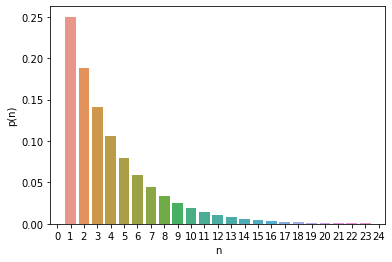
\includegraphics[width=\columnwidth]{plot.png}
    \caption{PMF of $X$  }
    \label{beta}
\end{figure}

\end{document}
